%%%%%%%%%%%%%%%%%%%%%%%%%%%%%%%%%%%%%%%%%
% Short Sectioned Assignment
% LaTeX Template
% Version 1.0 (5/5/12)
%
% This template has been downloaded from:
% http://www.LaTeXTemplates.com
%
% Original author:
% Frits Wenneker (http://www.howtotex.com)
%
% License:
% CC BY-NC-SA 3.0 (http://creativecommons.org/licenses/by-nc-sa/3.0/)
%
%%%%%%%%%%%%%%%%%%%%%%%%%%%%%%%%%%%%%%%%%

%----------------------------------------------------------------------------------------
%	PACKAGES AND OTHER DOCUMENT CONFIGURATIONS
%----------------------------------------------------------------------------------------

\documentclass[paper=a4, fontsize=11pt]{scrartcl} % A4 paper and 11pt font size

\usepackage[T1]{fontenc} % Use 8-bit encoding that has 256 glyphs
\usepackage{fourier} % Use the Adobe Utopia font for the document - comment this line to return to the LaTeX default
\usepackage[english]{babel} % English language/hyphenation
\usepackage{amsmath,amsfonts,amsthm} % Math packages
\usepackage{enumerate}
\usepackage{lipsum} % Used for inserting dummy 'Lorem ipsum' text into the template
\usepackage{sectsty} % Allows customizing section commands
\allsectionsfont{\centering \normalfont\scshape} % Make all sections centered, the default font and small caps
\sectionfont{\raggedright}
\usepackage[english]{babel}
\usepackage{mathtools}
\usepackage{graphicx}
\graphicspath{ {img/} }
\DeclareGraphicsExtensions{.png,.jpg}
\usepackage{color}
\usepackage{pbox}

\usepackage{fancyhdr} % Custom headers and footers
\pagestyle{fancyplain} % Makes all pages in the document conform to the custom headers and footers
\fancyhead{} % No page header - if you want one, create it in the same way as the footers below
\fancyfoot[L]{} % Empty left footer
\fancyfoot[C]{} % Empty center footer
\fancyfoot[R]{\thepage} % Page numbering for right footer
\renewcommand{\headrulewidth}{0pt} % Remove header underlines
\renewcommand{\footrulewidth}{0pt} % Remove footer underlines
\setlength{\headheight}{13.6pt} % Customize the height of the header

\numberwithin{equation}{section} % Number equations within sections (i.e. 1.1, 1.2, 2.1, 2.2 instead of 1, 2, 3, 4)
\numberwithin{figure}{section} % Number figures within sections (i.e. 1.1, 1.2, 2.1, 2.2 instead of 1, 2, 3, 4)
\numberwithin{table}{section} % Number tables within sections (i.e. 1.1, 1.2, 2.1, 2.2 instead of 1, 2, 3, 4)

\setlength\parindent{0pt} % Removes all indentation from paragraphs - comment this line for an assignment with lots of text

%----------------------------------------------------------------------------------------
%	TITLE SECTION
%----------------------------------------------------------------------------------------

\newcommand{\horrule}[1]{\rule{\linewidth}{#1}} % Create horizontal rule command with 1 argument of height

\title{	
\normalfont \normalsize 
\textsc{National Taiwan University, \\ Graduate Institute of Biomedical Engineering and Bioinformatics} \\ [25pt] % Your university, school and/or department name(s)
\horrule{0.5pt} \\[0.4cm] % Thin top horizontal rule
\huge BEBI5009:\\Mathematical Modeling of System Biology \\ Homework 4 \\ % The assignment title
\horrule{2pt} \\[0.5cm] % Thick bottom horizontal rule
}

\author{Yi Hsiao\\R04945027} % Your name

\date{\normalsize\today} % Today's date or a custom date

\begin{document}

\maketitle % Print the title

\newpage
\section{}
Consider the reaction network
	\begin{gather*}
			A \xrightarrow{k_1} B + C \\
			B + C \xrightarrow{k_{-1}} A
	\end{gather*}
	\begin{enumerate}[a)]
		\item  Suppose that the system starts with two molecules of A, one molecule of B, and no molecules of C, that is ($N_A$,$N_B$, $N_C$) = (2, 1, 0). Determine the set of possible states the system can adopt and write the chemical master equation that describes the corresponding probability distribution.

		All possible states of ($N_A$,$N_B$, $N_C$) are (2, 1, 0), (1,2,1), (0,3,1). Corresponding chemical master equation is:
		\begin{align*}
			&\frac{d}{dt}P((2,1,0),t)= -2k_1P((2,1,0),t)+2k_{-1}P((1,2,1),t) \\
			&\frac{d}{dt}P((1,2,1),t)= -k_1P((1,2,1),t)-2k_{-1}P((1,2,1),t)+2k_1P((2,1,0),t)+6k_{-1}P((0,3,2),t)\\
			&\frac{d}{dt}P((0,3,2),t)= -6k_{-1}P((0,3,2),t) + k_1P((1,2,1),t)
		\end{align*}

		\item Take $k_1$ = 1 ($time^{-1}$) and $k_{-1}$ = 1 ($time^{-1}$), and solve for the steady-state probability distribution.

		At steady state,
		\begin{align*}
			&0= -2k_1P^{ss}((2,1,0),t)+2k_{-1}P^{ss}((1,2,1),t) \\
			&0= -k_1P^{ss}((1,2,1),t)-2k_{-1}P^{ss}((1,2,1),t)+2k_1P^{ss}((2,1,0),t)+6k_{-1}P^{ss}((0,3,2),t)\\
			&0= -6k_{-1}P^{ss}((0,3,2),t) + k_1P^{ss}((1,2,1),t)\\
			Also, &\quad P^{ss}((2,1,0),t)+P^{ss}((1,2,1),t)+P^{ss}((0,3,2),t)=1\\
			\Rightarrow & 0 = -2P^{ss}((2,1,0),t)+2P^{ss}((1,2,1),t)\\
			&0= -P^{ss}((1,2,1),t)-2P^{ss}((1,2,1),t)+2P^{ss}((2,1,0),t)+6P^{ss}((0,3,2),t)\\
			&0= -6P^{ss}((0,3,2),t) + P^{ss}((1,2,1),t)\\
			&P^{ss}((2,1,0),t)+P^{ss}((1,2,1),t)+P^{ss}((0,3,2),t)=1\\
			\Rightarrow & P^{ss}((2,1,0),t)=\frac{6}{13}, \quad P^{ss}((1,2,1),t)=\frac{6}{13}, \quad P^{ss}((0,3,2),t)=\frac{1}{13}
		\end{align*}

		\item  Simulate sample paths of $N_A$, $N_B$, and $N_C$ using stochastic simulation algorithm (SSA). Set the initial condition of $N_A$, $N_B$, and $N_C$=(2,1,0) or (10, 5, 0) or (100, 50, 0)
		\begin{align*}
			&R1: A \xrightarrow{} B + C \quad propensity: k_1N_A \\
			&R2: B + C \xrightarrow{} A \quad propensity: k_{-1}N_BN_C
		\end{align*}
		Note1: To calculate the waiting time, you will need to generate values of a random variable distributed according to an exponential distribution. You could simply generate a random variable U drawn from the uniform distribution on the unit interval (0, 1), and T=-ln(U)/$\lambda$ will be an exponential random variable, where $\lambda$ is the rate parameter of the exponential distribution. In this example, $\lambda$ would be the sum of the reaction propensities. \\
		Another way to generate exponential random number is to use Matlab function exprnd($\mu$), where $\mu$ is the mean of the exponential distribution $\mu$=1/$\lambda$. \\
		Note2: You might need to change the value of $k_1$ and $k_{-1}$ for different initial conditions due to the volume changes. Use ($k_1$, $k_{-1}$) = (1,1), ( 1, 1/5) and (1, 1/50) ($time^{-1}$) for I.C.= (2,1,0), (10, 5, 0) , and (100, 50, 0).

		The simulation result of $N_A$, $N_B$, and $N_C$=(2,1,0)\\
		\includegraphics[scale=0.3]{{c.1}.jpg}\\
		The simulation result of $N_A$, $N_B$, and $N_C$=(10, 5, 0)\\
		\includegraphics[scale=0.3]{{c.2}.jpg}\\
		The simulation result of $N_A$, $N_B$, and $N_C$=(100, 50, 0)\\
		\includegraphics[scale=0.3]{{c.3}.jpg}

		\item Set the initial condition of $N_A$, $N_B$, and $N_C$=(2, 1, 0). Analyzed the statistics of your ensemble, and compare to the steady state probability distribution in (b)

		The simulation result of an ensemble of 3 sample paths (the bold line represents the average behaviour):\\
		\includegraphics[scale=0.3]{{d.1}.jpg}\\
		The simulation result of an ensemble of 10 sample paths:\\
		\includegraphics[scale=0.3]{{d.2}.jpg}\\
		The simulation result of an ensemble of 100 sample paths:\\
		\includegraphics[scale=0.3]{{d.3}.jpg}
		\\As the ensemble size increases, the averaged behavior approaches the deterministic prediction. I sampled the distribution of states at 10, which is already at steady-state, but the probability distribution of $N_A$, $N_B$, and $N_C$=(2,1,0), (1,2,1), (0,3,2) are 0.01, 0.01, 0.98. It is quite different from the result we derived in (b). It may due to the simulation conducted in a discrete manner, and the boundary conditions that should be followed further constrained and modified the original behaviour of the system.



		\item Write down a deterministic model for the chemical reaction following the mass action law. Simulate the concentration changes of A, B C with the parameter $k_1$ = 1($s^{-1}$) and $k_{-1}$ = 1 ($mM^{-1}s^{-1}$). Set initial concentrations [A],[B],[C] as 2, 1, and 0mM. Compare simulation results in (c)

		According to the question, we can easily list following equations:
		\begin{align*}
			&\frac{d[A]}{dt} = -k_1[A] + k_{-1}[B][C]\\
			&\frac{d[B]}{dt} = k_1[A] - k_{-1}[B][C]\\
			&\frac{d[C]}{dt} = k_1[A] - k_{-1}[B][C]
		\end{align*}
		The simulation result is shown in following figure:\\
		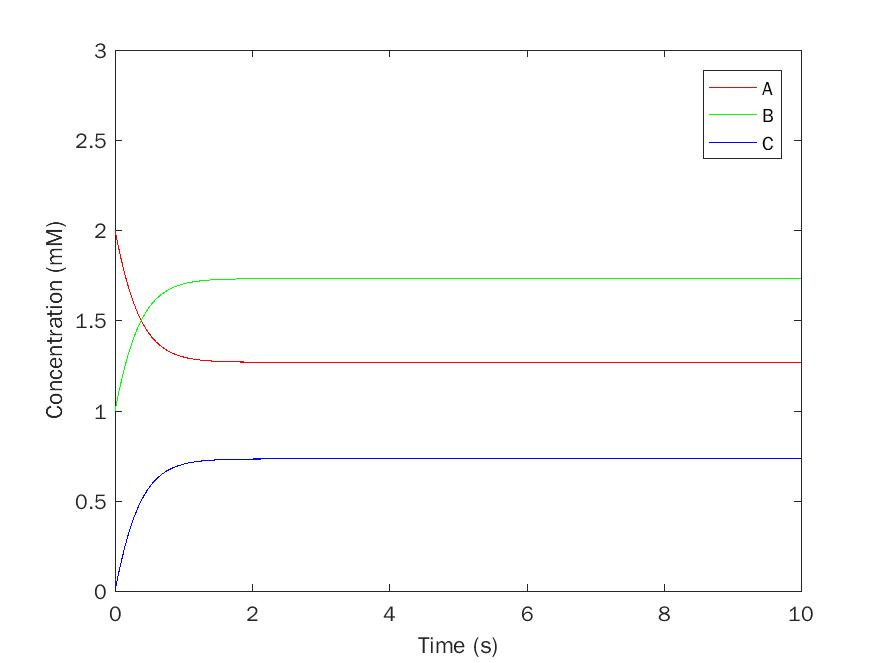
\includegraphics[scale=0.3]{e.jpg}\\
		Compared to the results obtained in (c), random behavior is not well-described by the deterministic simulation for small population size. Whereas it's a good description for large population size.

	\end{enumerate}


\end{document}